\documentclass[12pt]{article}
\usepackage[margin=1in]{geometry}
\usepackage{amsmath,amsthm,amssymb}

\usepackage[T1]{fontenc}
\usepackage{bigfoot} % to allow verbatim in footnote
\usepackage[numbered,framed]{matlab-prettifier}
\usepackage{filecontents}
\usepackage{graphicx}

\let\ph\mlplaceholder % shorter macro
\lstMakeShortInline"

\lstset{
  style              = Matlab-editor,
  basicstyle         = \mlttfamily,
  escapechar         = ",
  mlshowsectionrules = true,
}

\title{MAE 275 - Homework 2}
\author{John Karasinski}

\begin{document}
\maketitle

\section{Problem 1}
We can define the longitudinal and lateral linearized aircraft equations of motion. The longitudinal equations can be expressed as
\begin{equation}
\begin{split}
\Delta \dot{u} = &X_u \Delta u + X_w \Delta w - g\cos \theta_0 \Delta \theta + \sum\limits_{i=1}^n X_{\delta_i} \Delta \delta_i \\
\Delta \dot{w} = &\dfrac{Z_u}{1-Z_{\dot{w}}} \Delta u +
                  \dfrac{Z_w}{1-Z_{\dot{w}}} \Delta w +
                  \dfrac{Z_q + u_0}{1-Z_{\dot{w}}} \Delta q -
                  \dfrac{g\sin \theta_0}{1-Z_{\dot{w}}} \Delta \theta +
                  \dfrac{1}{1-Z_{\dot{w}}} \sum\limits_{i=1}^n Z_{\delta_i} \Delta \delta_i \\
\Delta \dot{q} = &\left[ M_u + \dfrac{M_{\dot{w}} Z_u}{1-Z_{\dot{w}}} \Delta u  \right] +
                  \left[ M_w + \dfrac{M_{\dot{w}} Z_w}{1-Z_{\dot{w}}} \Delta w  \right] +
                  \left[ M_q + \dfrac{M_{\dot{w}} (Z_q + u_0)}{1-Z_{\dot{w}}} \Delta q  \right] \\
                 & - \left[ \dfrac{M_{\dot{w}} g\sin \theta_0}{1-Z_{\dot{w}}} \Delta \theta  \right]
                   + \dfrac{M_{\dot{w}}}{1-Z_{\dot{w}}} \sum\limits_{i=1}^n Z_{\delta_i} \Delta \delta_i
                   + \sum\limits_{i=1}^n M_{\delta_i} \Delta \delta_i \\
\Delta \dot{\theta} = &\Delta q \\
\Delta \dot{h} = &-\Delta w + u_0 \Delta \theta \\
\end{split}
\label{long}
\end{equation}

\noindent or in state space form, with state variables $\Delta u, \Delta w, \Delta q, \Delta \theta, \Delta h $, as
\begin{equation*}
A =
\begin{bmatrix}
    X_u & X_w & 0 & -g \cos(\theta_0) & 0 \\
    \dfrac{Z_u}{1-Z_{\dot{w}}} & \dfrac{Z_w}{1-Z_{\dot{w}}} & \dfrac{Z_q + u_0}{1-Z_{\dot{w}}} & \dfrac{g\sin \theta_0}{1-Z_{\dot{w}}} & 0 \\
    M_u + \dfrac{M_{\dot{w}} Z_u}{1-Z_{\dot{w}}} & M_w + \dfrac{M_{\dot{w}} Z_w}{1-Z_{\dot{w}}} & M_q + \dfrac{M_{\dot{w}} (Z_q + u_0)}{1-Z_{\dot{w}}} & -\dfrac{M_{\dot{w}} g\sin \theta_0}{1-Z_{\dot{w}}} & 0 \\
    0 & 0 & 1 & 0 & 0 \\
    0 & -1 & 0 & u_0 & 0
\end{bmatrix}
\end{equation*}

\noindent Plugging in the data for the F-89 aircraft (Flight Condition 8901) on pages A3-A5 in the Appendix of "Aircraft Dynamics and Automatic Control" yields
\begin{equation*}
A =
\begin{bmatrix}
  -9.7000e-03  & +1.6000e-03  &           0  & -3.2200e+01 &           0 \\
  -9.5500e-02  & -1.4300e+00  & +6.6000e+02  &           0 &           0 \\
  +1.2415e-04  & -2.1641e-02  & -2.7780e+00  &           0 &           0 \\
            0  &           0  & +1.0000e+00  &           0 &           0 \\
            0  & -1.0000e+00  &           0  & +6.6000e+02 &           0 \\
\end{bmatrix}
\end{equation*}

\noindent The lateral equations can be expressed as
\begin{equation}
\begin{split}
\Delta \dot{v} = & Y_v\Delta v + Y_p\Delta p + \left[ Y_r - u_0 \right]\Delta r + g\cos\theta_0\Delta \varphi + \sum\limits_{i=1}^n Y_{\delta_i} \Delta \delta_i \\
\Delta \dot{p} = & L_v^\prime \Delta v + L_p^\prime \Delta p + L_r^\prime \Delta r + \sum\limits_{i=1}^n L_{\delta_i}^\prime \Delta \delta_i \\
\Delta \dot{r} = & N_v^\prime \Delta v + N_p^\prime \Delta p + N_r^\prime \Delta r + \sum\limits_{i=1}^n N_{\delta_i}^\prime \Delta \delta_i \\
\Delta \dot{\varphi} = &\Delta p + r\tan\theta_0\Delta r\\
\Delta \dot{\psi} = &r\sec\theta_0\Delta r\\
\end{split}
\label{lat}
\end{equation}

\noindent or in state space form, with state variables $\Delta v, \Delta p, \Delta r, \Delta \varphi, \Delta \psi $, as
\begin{equation*}
A =
\begin{bmatrix}
    Y_v & Y_p & \left[ Y_r-u_0 \right] & g\cos \theta_0 & 0 \\
    L_v^\prime & L_p^\prime & L_r^\prime & 0 & 0 \\
    N_v^\prime & N_p^\prime & N_r^\prime & 0 & 0 \\
    0 & 1 & \tan \theta_0 & 0 & 0 \\
    0 & 0 & \sec \theta_0 & 0 & 0
\end{bmatrix}\\
\end{equation*}

\noindent Plugging in the appropriate data
\begin{equation*}
A =
\begin{bmatrix}
  -8.2900e-02  &           0  & -6.6000e+02  & +3.2200e+01 &            0 \\
  -6.8939e-03  & -1.7000e+00  & +1.7200e-01  &           0 &            0 \\
  +5.1212e-03  & -6.5400e-02  & -8.9300e-02  &           0 &            0 \\
            0  & +1.0000e+00  &           0  &           0 &            0 \\
            0  &           0  & +1.0000e+00  &           0 &            0 \\
\end{bmatrix}
\end{equation*}

\newpage
\section{Problem 2}
\subsection{Longitudinal}
\noindent The following MATLAB command is called to identify the characteristic roots and eigenvector elements
\begin{filecontents*}{code.m}
[v, d] = eig(A);
\end{filecontents*}
\lstinputlisting[]{code.m}

\noindent resulting in two complex pairs of eigenvalues
\begin{equation*}
\begin{split}
d_1 =& -2.1043e+0 \pm i 3.7184e+0 \mbox{ (Short-Period Mode)} \\
d_2 =& -4.5114e-3 \pm i 6.2756e-2 \mbox{ (Phugoid Mode)}\\
\end{split}
\end{equation*}

\noindent and their associated eigenvectors
\begin{equation*}
\begin{split}
v_1 = [-7.3823e-3 & \mp i 6.3366e-3, \\
       -9.9688e-1 &,  \\
        1.0175e-3 & \mp i 5.6172e-3, \\
       -1.2615e-3 & \pm i 4.4029e-4, \\
        4.0253e-2 & \mp i 6.6963e-2] \\
v_2 = [ 4.8201e-2 & \pm i 7.1255e-3, \\
       -4.8242e-4 & \mp i 8.0362e-5,  \\
        5.9403e-6 & \pm i 8.1160e-7,  \\
        6.0964e-6 & \mp i 9.5094e-5, \\
       -9.9881e-1 &].
\end{split}
\end{equation*}

\noindent Before exciting these modes, the rest of the state space system must be defined. The longitudinal A matrix from above is used, along with B, C, and D matrices defined as
\begin{filecontents*}{code.m}
B = [0; 0; 0; 0; 0];

C = [[1, 0, 0, 0, 0];
     [0, 1/u_0, 0, 0, 0];
     [0, 0, 1, 0, 0];
     [0, 0, 0, 1, 0];
     [0, 0, 0, 0, 1]];

D = [0; 0; 0; 0; 0];
\end{filecontents*}
\lstinputlisting[]{code.m}

\noindent Finally, the initial state can be defined and the initial command can be run by
\begin{filecontents*}{code.m}
i1 = real(v(:,1));
initial(A, B, C, D, i1, 5)
\end{filecontents*}
\lstinputlisting[]{code.m}

\noindent and results in the following figures
\begin{figure}[h]
\begin{center}
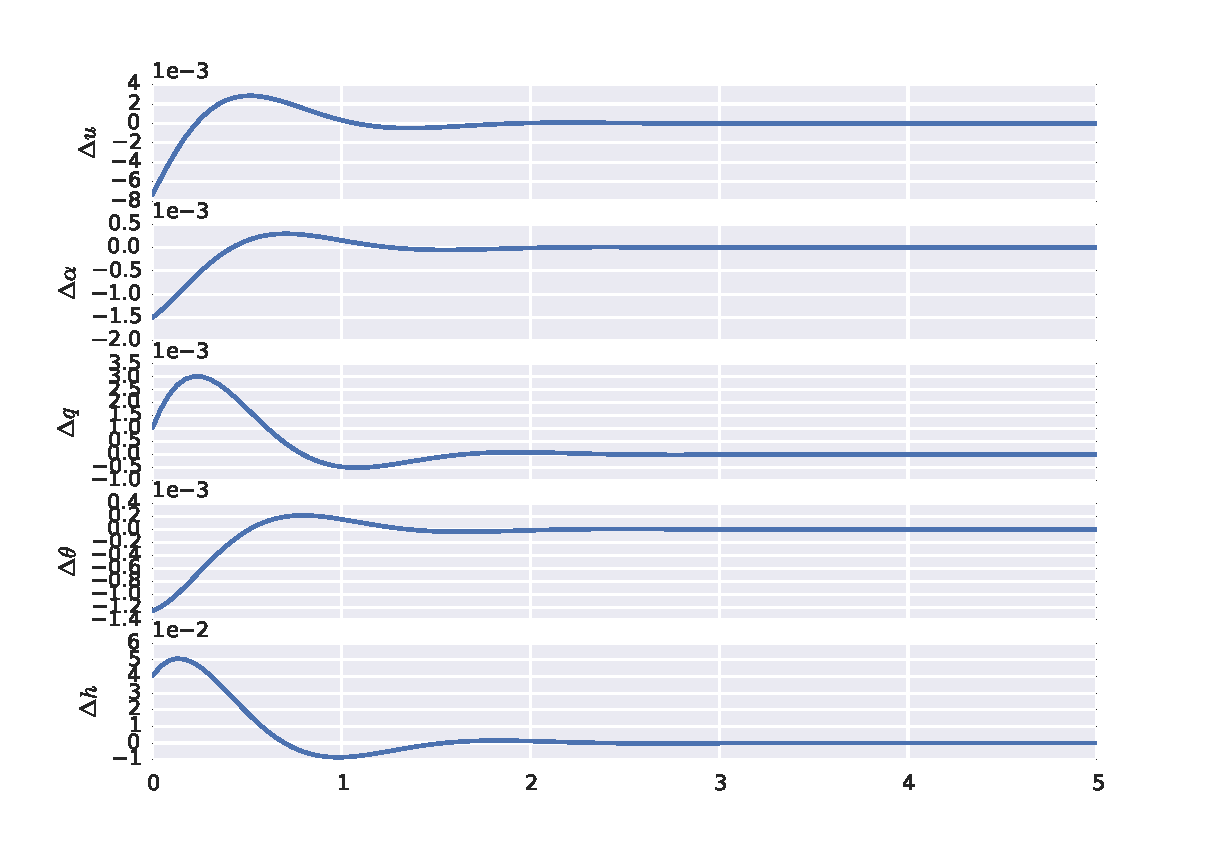
\includegraphics[width=0.85\textwidth]{figures/LongI2.pdf}
\caption{Initial response to eigenvector $v_1$}
\label{}
\end{center}
\end{figure}

\begin{figure}[h]
\begin{center}
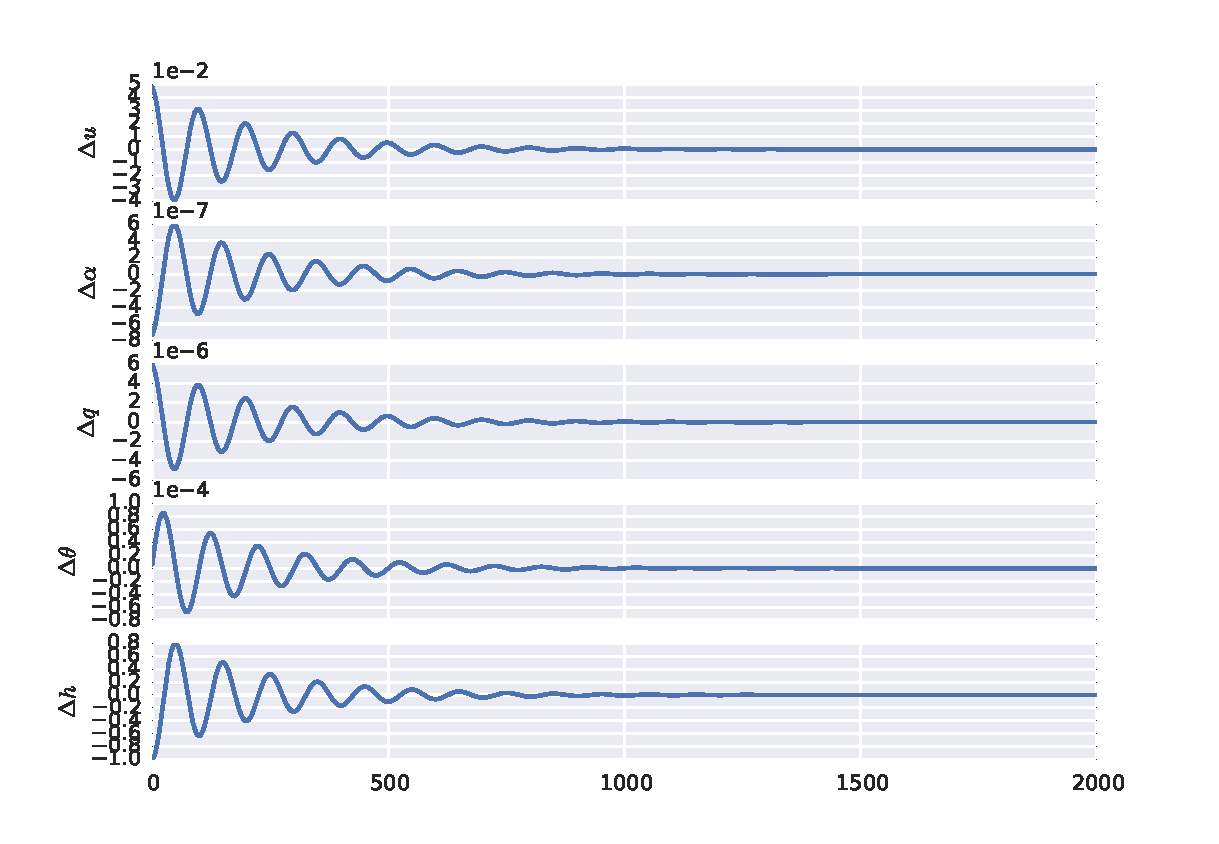
\includegraphics[width=0.85\textwidth]{figures/LongI4.pdf}
\caption{Initial response to eigenvector $v_2$}
\label{}
\end{center}
\end{figure}

\clearpage
\subsection{Lateral}
\noindent The lateral eigenvalues are identified as
\begin{equation*}
\begin{split}
d_1 = -1.7808e+0 & \mbox{ (Roll Convergence Mode)}\\
d_2 = +1.3590e-3 & \mbox{ (Slightly Unstable Spiral Mode)}\\
d_3 = -4.6373e-2 &\pm i 1.8779e+0 \mbox{ (Dutch Roll Mode)} \\
\end{split}
\end{equation*}

\noindent and their associated eigenvectors
\begin{equation*}
\begin{split}
v_1 = [-9.9531e-1 &, \\
       -8.4376e-2 &, \\
       -2.4891e-4 &, \\
       +4.7381e-2 &, \\
       +1.3977e-4 &] \\
v_2 = [-2.4525e-2 &, \\
       -3.7916e-5 &, \\
       -1.3581e-3 &, \\
       -2.7900e-2 &, \\
       -9.9931e-1 &] \\
v_3 =  +9.9999e-1 &, \\
       -1.9651e-3 & \pm i 1.9409e-3, \\
       -3.6905e-6 & \mp i 2.7955e-3, \\
       +1.0587e-3 & \pm i 1.0203e-3, \\
       -1.4877e-3 & \pm i 3.8701e-5] \\
\end{split}
\end{equation*}

\noindent Before exciting these modes, the rest of the state space system must be defined. The lateral A matrix from above is used, along with B, C, and D matrices defined as
\begin{filecontents*}{code.m}
B = [0; 0; 0; 0; 0];

C = [[1/u_0, 0, 0, 0, 0];
     [0, 1, 0, 0, 0];
     [0, 0, 1, 0, 0];
     [0, 0, 0, 1, 0];
     [0, 0, 0, 0, 1]];

D = [0; 0; 0; 0; 0];
\end{filecontents*}
\lstinputlisting[]{code.m}

\noindent Exciting each of these modes with the appropriate eigenvector results in
\begin{figure}[h]
\begin{center}
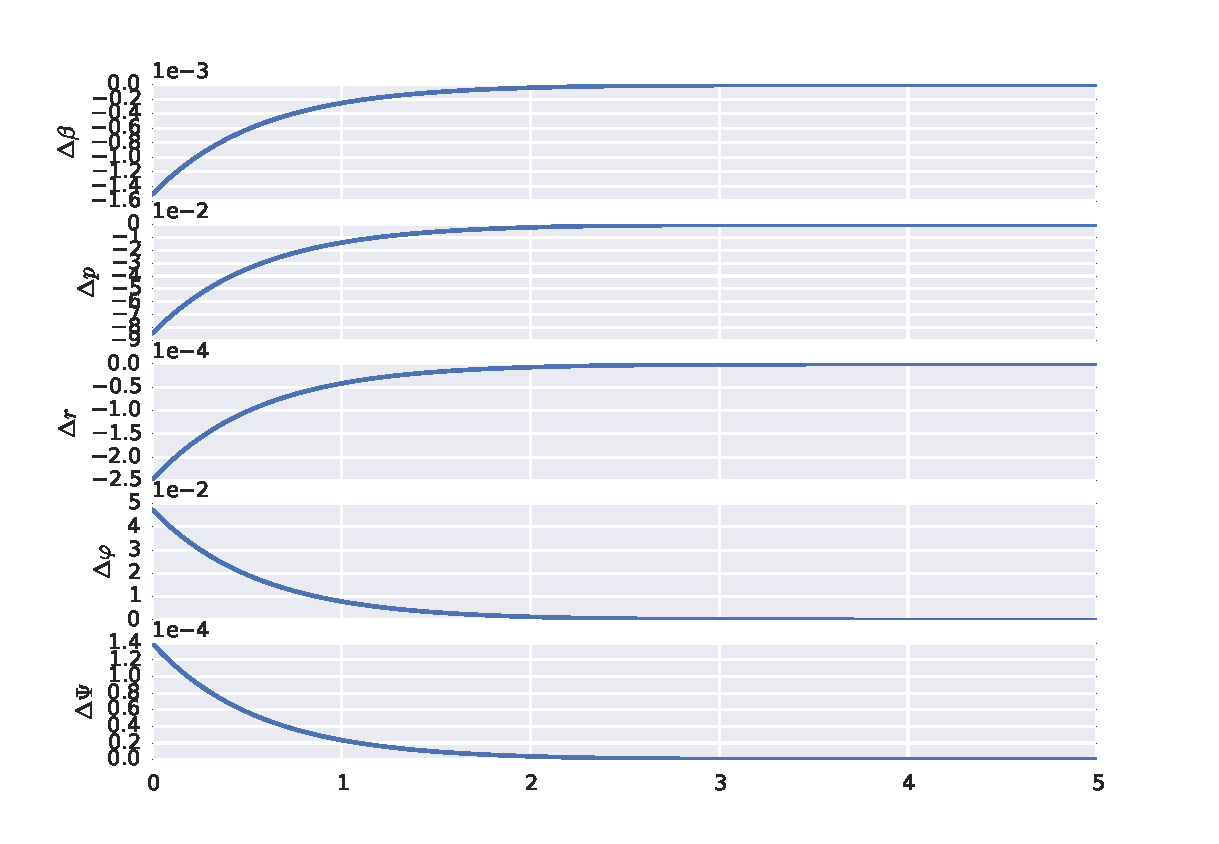
\includegraphics[width=0.85\textwidth]{figures/LatI2.pdf}
\caption{Initial response to eigenvector $v_1$}
\label{}
\end{center}
\end{figure}

\begin{figure}[h]
\begin{center}
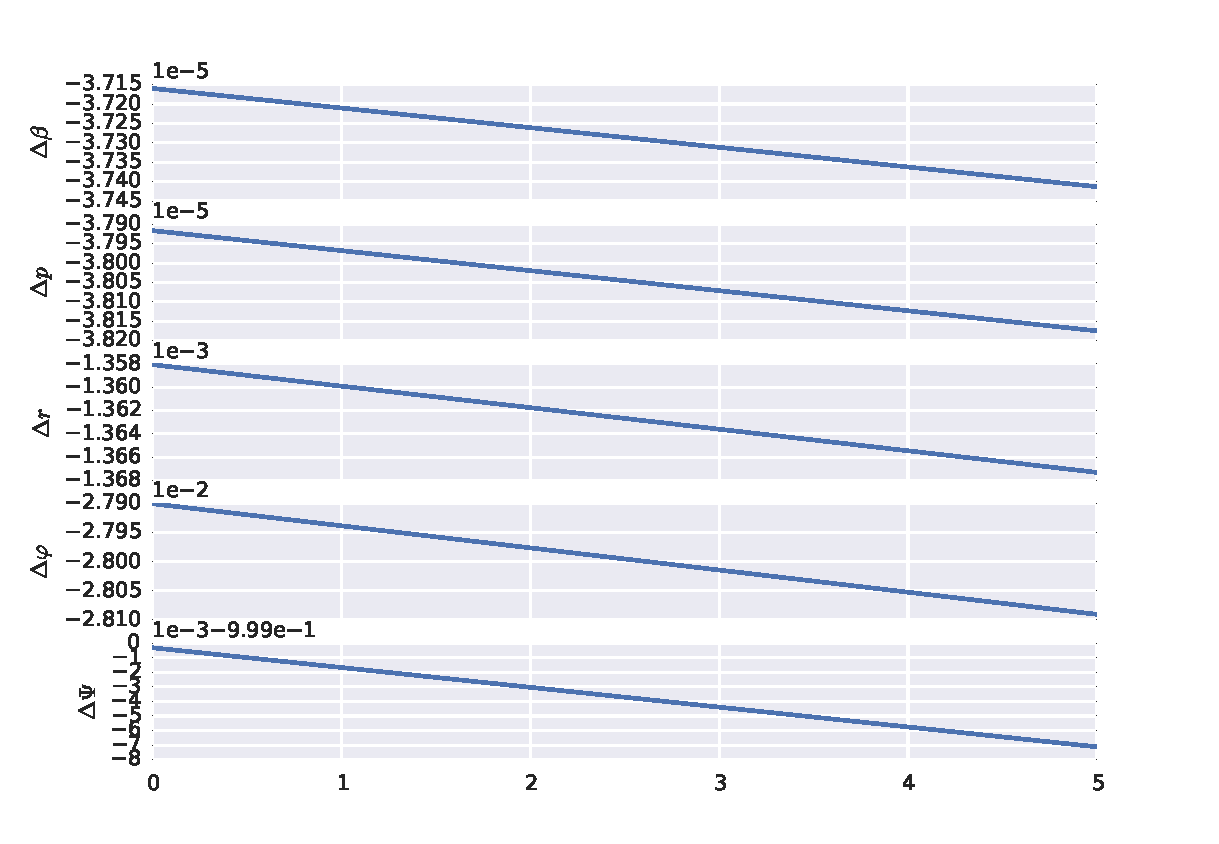
\includegraphics[width=0.85\textwidth]{figures/LatI3.pdf}
\caption{Initial response to eigenvector $v_2$}
\label{}
\end{center}
\end{figure}

\begin{figure}[h]
\begin{center}
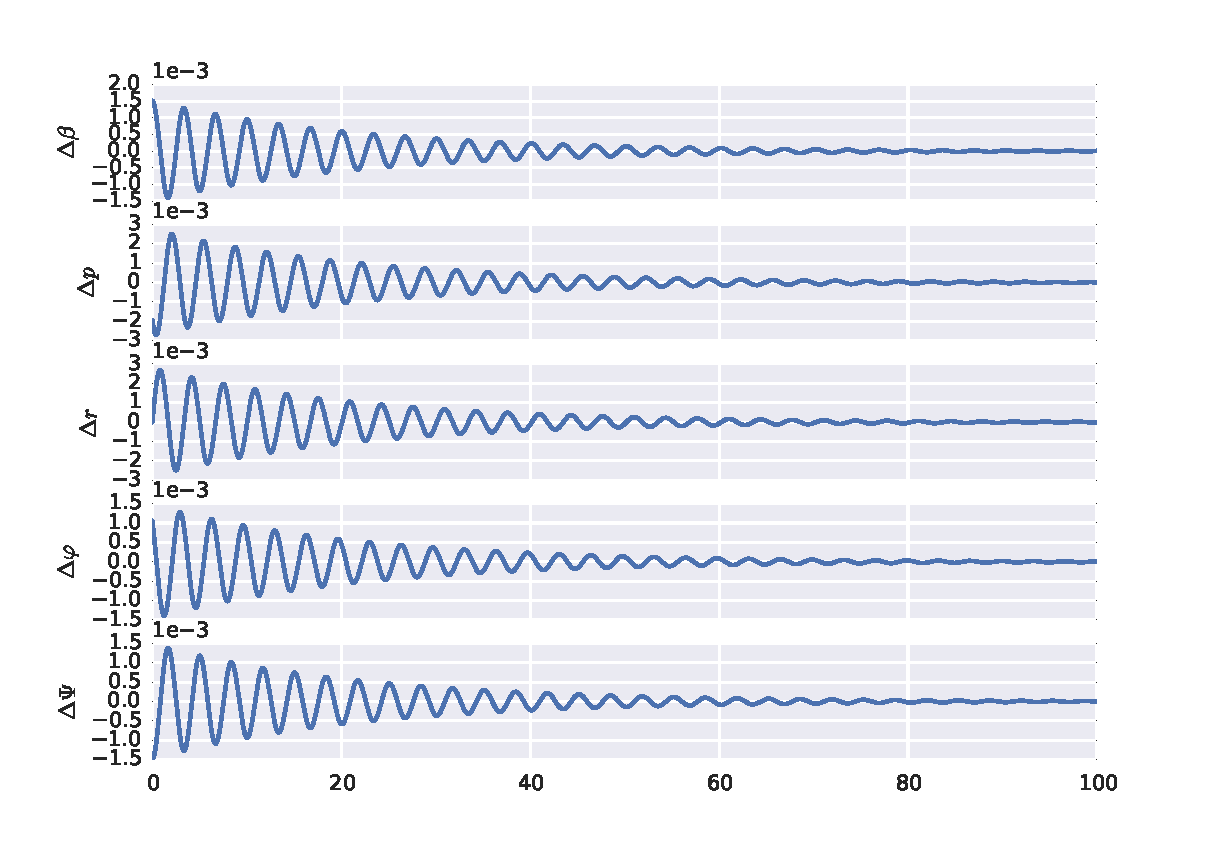
\includegraphics[width=0.85\textwidth]{figures/LatI4.pdf}
\caption{Initial response to eigenvector $v_3$}
\label{}
\end{center}
\end{figure}

\clearpage
\section{Problem 3}
\subsection{Longitudinal}
A control input to the elevators, $\Delta \delta_e$, can be found by solving Equation~\ref{long}, resulting in a B matrix,
\begin{equation*}
B =
\begin{bmatrix}
   X_{\delta_e} \\
   \dfrac{Z_{\delta_e}}{1-Z_{\dot{w}}} \\
   \dfrac{M_{\dot{w}} Z_{\delta_e}}{1-Z_{\dot{w}}} + M_{\delta_e} \\
   0 \\
   0 \\
\end{bmatrix}
=
\begin{bmatrix}
   0 \\
   -6.9800e+1 \\
   -2.6009e+1 \\
   0 \\
   0 \\
\end{bmatrix}
\end{equation*}

\noindent After defining the C and D matrices, we can find the resulting transfer function with the following commands
\begin{filecontents*}{code.m}
C=[0 0 0 1 0];
D = 0;

[n, d] = ss2tf(A, B, C, D);
minreal(zpk(tf(n,d)))
\end{filecontents*}
\lstinputlisting[]{code.m}

\noindent which results in
\begin{filecontents*}{code.m}
             -26.009 (s+1.372) (s+0.009813)
  ---------------------------------------------------
  (s^2 + 0.009023s + 0.003959) (s^2 + 4.209s + 18.25)
\end{filecontents*}
\lstinputlisting[]{code.m}
\noindent yielding
\begin{equation*}
\begin{split}
A_{\theta} =& -26.009 \\
1/T_{\theta_1} =& +0.009813 \\
1/T_{\theta_2} =& +1.372,
\end{split}
\end{equation*}

\noindent which compare quite well with the values found on page A-5,
\begin{equation*}
\begin{split}
A_{\theta} =& -26.1 \\
1/T_{\theta_1} =& +0.0098 \\
1/T_{\theta_2} =& +1.372
\end{split}
\end{equation*}

\subsection{Lateral}
\noindent A control input to the aileron, $\Delta \delta_a$, can be found by solving Equation~\ref{lat}, resulting in a B matrix,
\begin{equation*}
B =
\begin{bmatrix}
   Y_{\delta_a} \\
   L_{\delta_a}^\prime \\
   N_{\delta_a}^\prime \\
   0 \\
   0 \\
\end{bmatrix}
=
\begin{bmatrix}
   0 \\
   2.7300e+01 \\
   3.9500e-01 \\
   0 \\
   0 \\
\end{bmatrix}
\end{equation*}

\noindent Defining the C and D matrices the same as above, we can find the resulting transfer function
\begin{filecontents*}{code.m}
           27.3 (s^2 + 0.1747s + 3.453)
  -----------------------------------------------
  (s+1.781) (s-0.001359) (s^2 + 0.09275s + 3.529)
\end{filecontents*}
\lstinputlisting[]{code.m}
\noindent yielding
\begin{equation*}
\begin{split}
A_{\theta} =& +27.3 \\
\zeta_{\varphi} =& +4.7007e-02\\
\omega_{\varphi} =& -1.8582e+00,
\end{split}
\end{equation*}
\noindent which compare quite well with the values found on page A-5,
\begin{equation*}
\begin{split}
A_{\theta} =& +27.3 \\
\zeta_{\varphi} =& +0.047\\
\omega_{\varphi} =& -1.86
\end{split}
\end{equation*}

\newpage
\section{Problem 4}
The response to a step control input of $\Delta \delta_e = 5/57.3$ rad can be for $\Delta \theta$ and $\Delta h$. Two responses were seen, a phugoid,
\begin{figure}[h!]
\begin{center}
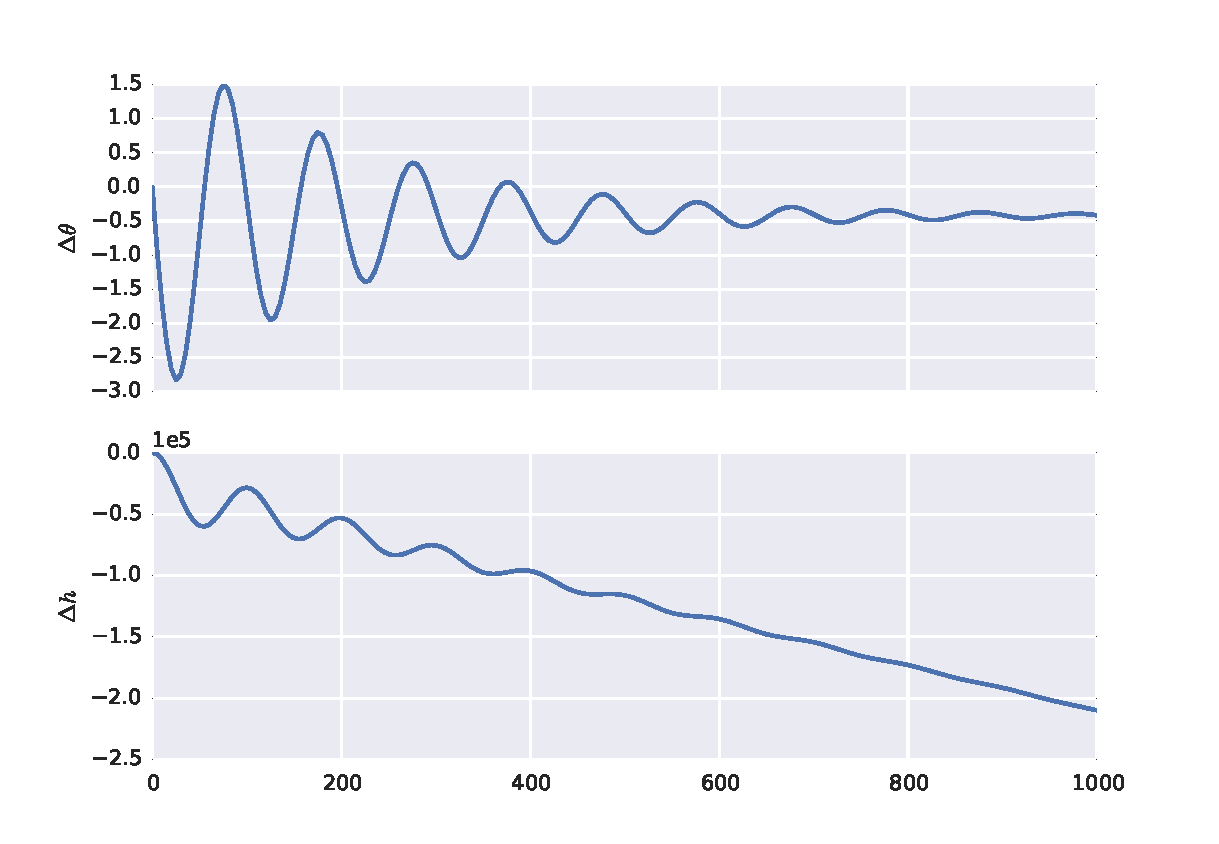
\includegraphics[width=0.7\textwidth]{figures/LongStepLong.pdf}
\caption{Phugoid response to step input}
\label{}
\end{center}
\end{figure}

\noindent and a short-period response which manifests as a small oscillation in $\Delta \theta$
\begin{figure}[h!]
\begin{center}
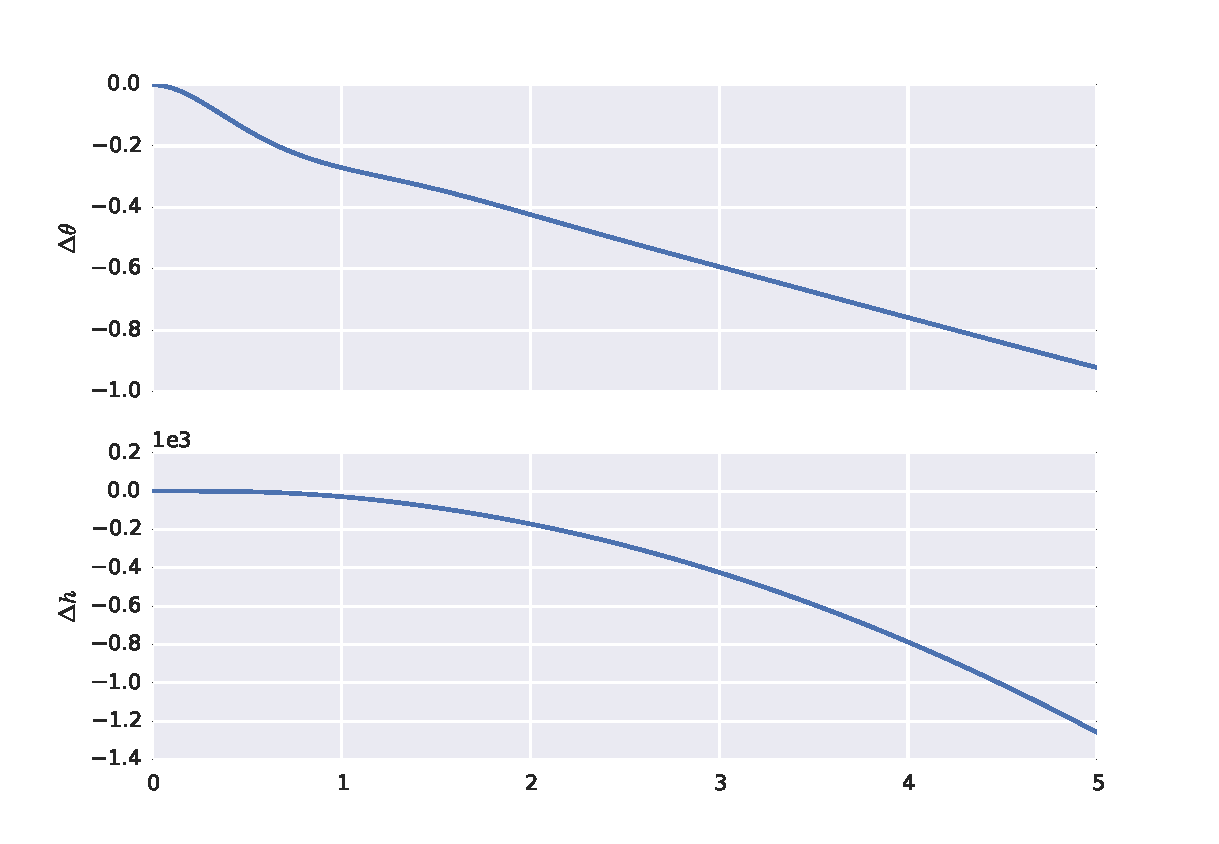
\includegraphics[width=0.7\textwidth]{figures/LongStepShort.pdf}
\caption{Short-period response to step input}
\label{}
\end{center}
\end{figure}

\clearpage
\noindent Similarly, the response to a step control input of $\Delta \delta_a = 5/57.3$ rad can be seen for $\Delta \varphi$ and $\Delta r$
\begin{figure}[h!]
\begin{center}
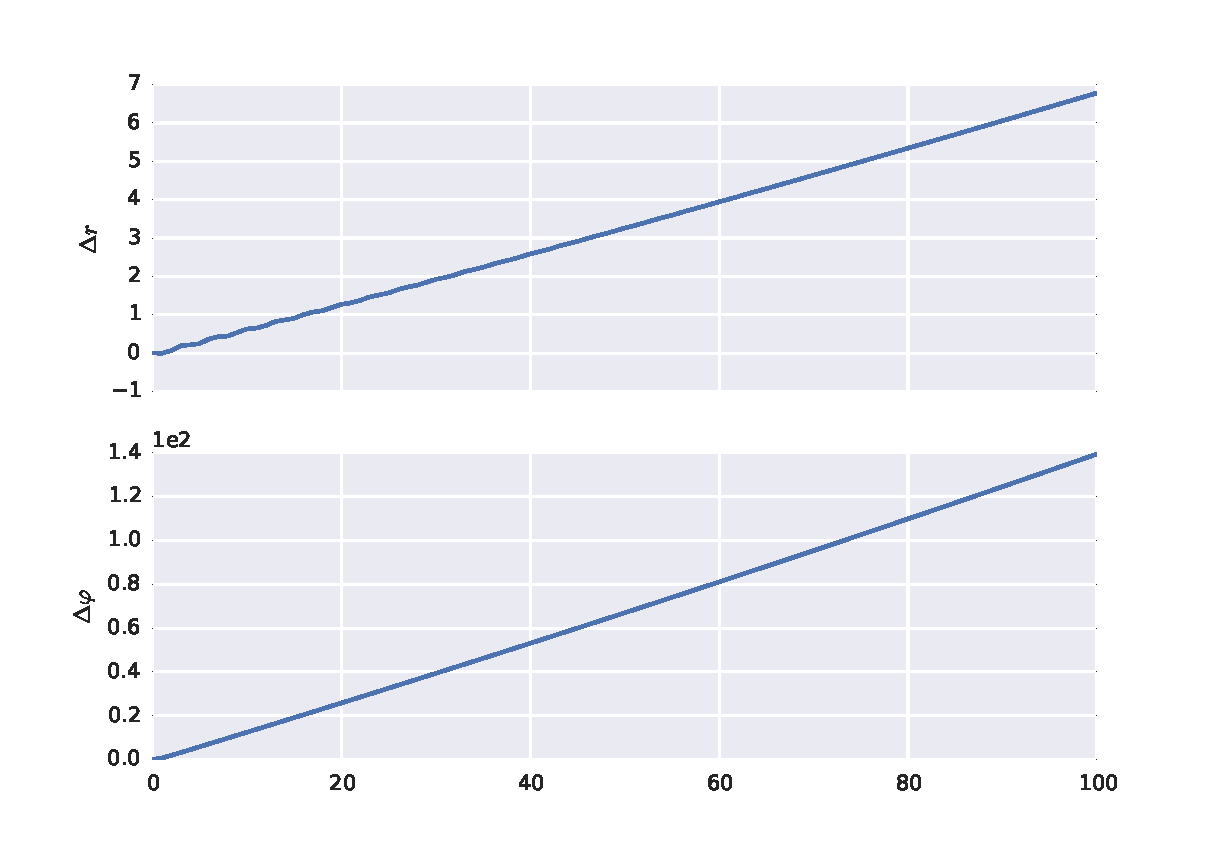
\includegraphics[width=0.7\textwidth]{figures/LatStep.pdf}
\caption{Step response to a step input in $\Delta \delta_a$}
\label{}
\end{center}
\end{figure}

\newpage
\appendix

\begin{figure}
\begin{equation*}
  \begin{split}
  % Basic Simulation Parameters
  h &= 20000 \\
  M &= 0.638 \\
  g &= 32.2 \\
  \theta_0 &= 0 \\
  u_0 &= 660 \\
  \end{split}
\end{equation*}
  \caption{Basic Simulation Parameters}
\end{figure}

\begin{figure}
\begin{equation*}
  \begin{split}
  % %% Longitudinal
  X_u &= -0.0097 \\
  X_w &= 0.0016 \\
  X_{\delta_e} &= 0 \\
  \\
  Z_u &= -0.0955 \\
  Z_{\dot{w}} &= 0 \\
  Z_w &= -1.43 \\
  Z_{\delta_e} &= -69.8 \\
  \\
  M_u &= 0 \\
  M_{\dot{w}} &= -0.0013 \\
  M_w &= -0.0235 \\
  M_q &= -1.92 \\
  M_{\delta_e} &= -26.1 \\
  \\
  % Assumed to be zero}
  Z_q &= 0 \\
  \end{split}
\quad\quad
\quad\quad
  \begin{split}
  %% Lateral
  Y_v &= -0.0829 \\
  Y_{\delta_a} &= 0 \\
  \\
  L_p^\prime &= -1.70 \\
  L_r^\prime &= 0.172 \\
  L_{\delta_a}^\prime &= 27.3 \\
  L_{\beta}^\prime &= -4.55 \\
  L_v^\prime &= \dfrac{L_{\beta}^\prime}{u_0} =-0.0069 \\
  \\
  N_p^\prime &= -0.0654 \\
  N_r^\prime &= -0.0893 \\
  N_{\delta_a}^\prime &= 0.395 \\
  N_{\beta}^\prime &= 3.38 \\
  N_v^\prime &= \dfrac{N_{\beta}^\prime}{u_0} = 0.0051 \\
  \\
  % Assumed to be zero
  Y_p &= 0 \\
  Y_r &= 0 \\
  \end{split}
\end{equation*}
  \caption{Longitudinal and Lateral Simulation Parameters}
\end{figure}

\end{document}
